\documentclass{beamer}
\usepackage[T1]{fontenc}
\usepackage[utf8]{inputenc}
\usepackage{lmodern}
\usepackage[brazil]{babel}
\usepackage{graphicx}
\usepackage{caption}
\usepackage{subcaption}

\captionsetup{compatibility=false}

\usetheme{JuanLesPins}
\useoutertheme[subsection=false]{miniframes}

\setbeamertemplate{frametitle}[default][center]
\title{
       \textbf{Seu Programa É Saudável?} \\
      }
\subtitle{
		\textbf{Virada Científica - CCSL}
		}
\author{Diego Martinez\\
        Rafael Manzo
       }

\begin{document}

\maketitle

\section{Introdução}

\begin{frame}
  \frametitle{Programas}
  \framesubtitle{}

  \begin{itemize}
    \item Todo programa possui um código fonte
    \begin{itemize}
      \item Código fonte é um conjunto de comandos que definem o que o progama faz
    \end{itemize}
    \item Escrever código \textbf{não} é uma ciência exata
  \end{itemize}

\end{frame}

\begin{frame}
  \frametitle{Programas bons}
  \framesubtitle{}

  O código pode ser bem escrito, resultando em um programa melhor.
  \begin{figure}
    \begin{center}
      
\includegraphics[height=.5\textheight]{images/linux.png}
    \end{center}
  \end{figure}
\end{frame}

\begin{frame}
  \frametitle{Programas ruins}
  \framesubtitle{}

  O programa pode ser ruim, provavelmente resultado de um código mal escrito.
  \begin{figure}
    \begin{center}
      
\includegraphics[height=.5\textheight]{images/windows.jpg}
    \end{center}
  \end{figure}
\end{frame}

\section{Métricas}
\begin{frame}
  \frametitle{Como sabemos se um programa é bom ou ruim?}
  Do ponto de vista do usuário:
  \begin{itemize}
    \item Se o programa produz os resultados esperados
    \item Se é rápido
    \item Se é fácil de usar
  \end{itemize}

  Do ponto de vista do programador:
  \begin{itemize}
    \item Se é fácil de entender o que está escrito
    \item Se tem pouca duplicação
    \item Se a estrutura faz sentido
  \end{itemize}

  \begin{block}{Métricas}
    Tanto usuários quanto programadores usam métricas para avaliar a qualidade de um programa.
  \end{block}
\end{frame}


\begin{frame}
  \frametitle{Importância das métricas}

  Para o programador, métricas são importantes pois:
  \begin{itemize}
    \item Auxiliam no controle da qualidade
    \item Indicam trechos que podem ter problemas
    \item São rápidas de serem calculadas
  \end{itemize}
\end{frame}

\begin{frame}
  \frametitle{Saúde de um programa}

  Avaliar a qualidade de um programa é análogo a fazer um \textit{checkup}.
  \begin{itemize}
    \item Fazemos um exame que nos dê indicadores relevantes sobre nossa saúde
    \item O médico interpreta os resultados e nos dá o diagnóstico
    \item Damos mais atenção ao que pode estar errado
    \item Se houver necessidade, fazemos mais exames para descobrir a natureza do problema
  \end{itemize}
\end{frame}

\begin{frame}
  \frametitle{O que normalmente medimos?}

  No nosso corpo, medimos:
  \begin{itemize}
    \item Quantidade de glicose no sangue
    \item Pressão
    \item Batimentos cardíacos
  \end{itemize}

  Em um programa, medimos:
  \begin{itemize}
    \item Linhas de código
    \item Nível de responsabilidade (coesão)
    \item Acoplamento
  \end{itemize}
\end{frame}

\section{Mezuro}
\begin{frame}
  \frametitle{Mezuro}
  \begin{figure}
    \begin{flushleft}
    \begin{center}
    \includegraphics[width=4cm, height=1.1cm]{images/logo-mezuro.png}
    \end{center}

      \label{fig:logo-mezuro}
    \end{flushleft}
  \end{figure}

  Sistema que faz \textit{checkups} periódicos no código fonte de um programa.
  \begin{itemize}
    \item Faz um exame e procura por indicadores de qualidade
    \item Interpreta os resultados e apresenta um diagnóstico
    \item Aponta os trechos que podem ter problemas
  \end{itemize}

  \begin{block}{Observação}
    Se mais exames forem necessários para investigar mais a fundo um possível problema,
    o próprio programador terá que olhar o código que escreveu.
  \end{block}
\end{frame}

\begin{frame}
  \frametitle{Exemplo de diagnóstico do Mezuro}
  \begin{figure}
    \begin{flushleft}
    \begin{center}
    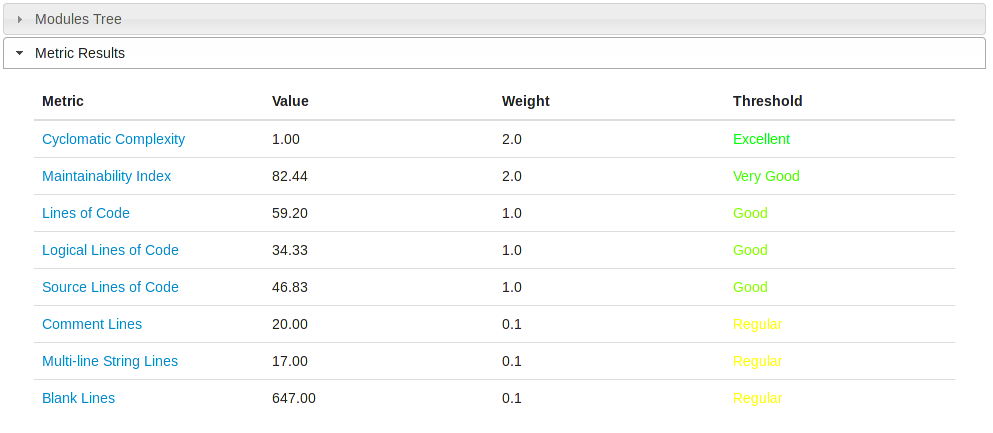
\includegraphics[width=10.5cm, height=6cm]{images/metric_results.png}
    \end{center}

      \label{fig:logo-mezuro}
    \end{flushleft}
  \end{figure}
\end{frame}

\begin{frame}
  \frametitle{Conheça-nos!}

  \begin{itemize}
    \item Site oficial: \url{http://mezuro.org}
    \item Código fonte: \url{https://github.com/mezuro}
    \item Lista de e-mails: mezuro@librelist.com
    \item Canal no IRC: \#mezuro
  \end{itemize}
\end{frame}

\begin{frame}
  \frametitle{Dúvidas?}
  \begin{figure}
    \begin{flushleft}
    \begin{center}
    
\includegraphics[width=10.5cm, height=6cm]{images/questions.jpg}
    \end{center}

      \label{fig:logo-mezuro}
    \end{flushleft}
  \end{figure}
\end{frame}

\end{document}
